\documentclass[a4paper, 10pt]{article}
\usepackage{amsmath}
\usepackage{fancyhdr}
\usepackage{float}
\usepackage[a4paper, left=1in, right=1in, top=1in, bottom=1in]{geometry} % Adjust margins
\usepackage{graphicx}
\usepackage{listings}
\usepackage{matlab-prettifier}
\usepackage{physics}
\usepackage{siunitx}

\lhead{}
\rhead{ECE 456 Problem Set 1}
\headheight 15pt
\pagestyle{fancy}

\begin{document}
\begin{titlepage}
    \vspace*{\fill}
    \begin{center}
        \Huge\textbf{ECE 456 Problem Set 1:\\} The Basics of Electron Flow in Nanodevices\\
        \vspace{1cm}
        \Large Omar Mahmoud, Nasif Qadri\\
        \vspace{0.5cm}
        \normalsize \today
    \end{center}
    \vspace*{\fill}
\end{titlepage}

% --------------------
% Problem 1a
% --------------------
\section{Current with a Lorentzian Density of States}

\subsection{Alternative Form}
% Original Equations
Given the following equations for the number of channel electrons and current in a nanodevice
\begin{equation}
    N = \int_{-\infty}^{\infty} \frac{\gamma_1 f_1(E) + \gamma_2 f_2(E)}{\gamma_1 + \gamma_2} D(E-U) \dd{E}
\end{equation}
\begin{equation}
    I = \frac{q}{\hbar}\frac{\gamma_1 \gamma_2}{\gamma_1 + \gamma_2}\int_{-\infty}^{\infty}[f_1(E) - f_2(E)]D(E-U) \dd{E}
\end{equation}\\
% Manipulation Steps
These equations can be manipulated to be easier to code into MATLAB. Firstly, change the variable of integration to $E' = E - U$. This can be manipulated to recieve
\begin{align*}
	&E' = E - U\\
	&E = E' + U\\
	&dE' = dE
\end{align*}
Originally $E: -\infty \rightarrow \infty$, however, since subtracting a constant doesn't change infinity
\[
    E': -\infty \rightarrow \infty
\]
% Final Equations
Hence, substituting for $E = E' + U$ and replacing $E' \rightarrow E$ produces
\begin{equation}
    N = \int_{-\infty}^{\infty} \frac{\gamma_1 f_1(E+U) + \gamma_2 f_2(E+U)}{\gamma_1 + \gamma_2} D(E) \dd{E}
\end{equation}
\begin{equation}
    I = \frac{q}{\hbar}\frac{\gamma_1 \gamma_2}{\gamma_1 + \gamma_2}\int_{-\infty}^{\infty}[f_1(E+U) - f_2(E+U)]D(E) \dd{E}
\end{equation}

\subsection{Solving the Equations Self-Consistently}

% --------------------
% Problem 1b
% --------------------
Using the code in \verb|problem1.py| to calculate the values of $N$ and $I$ self-consistently produced the plots seen in Figure \ref{fig:1b_plots}.
\begin{figure}[H]
	\centering
	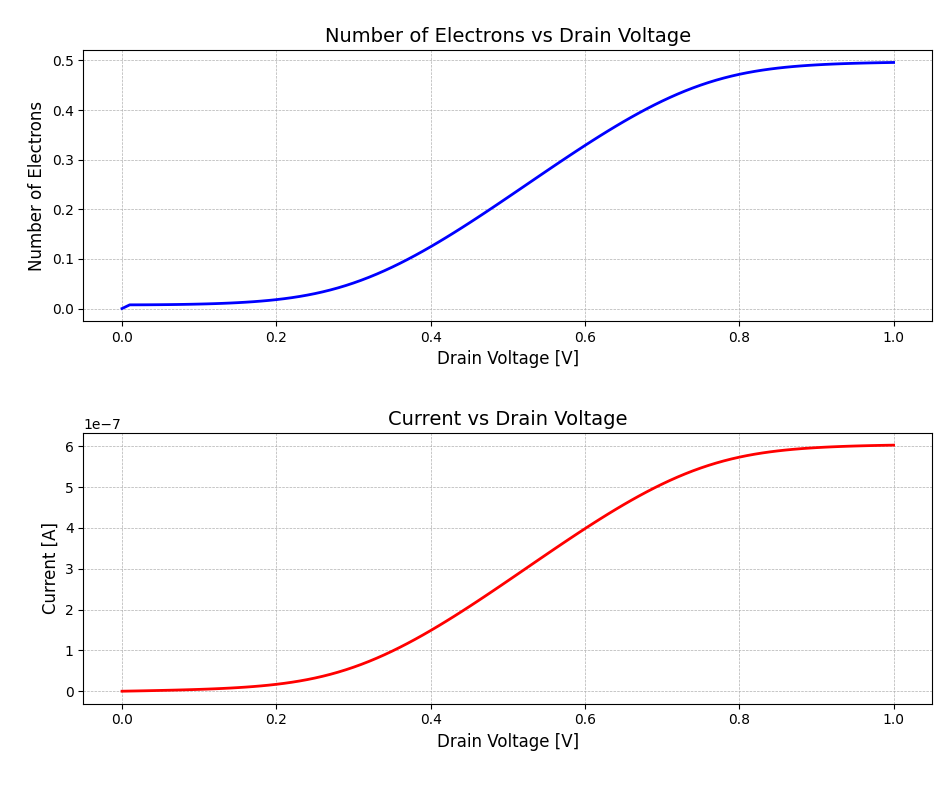
\includegraphics[width=10cm]{imgs/1b.png}
	\caption{Plot of the current ($I$) and number of electrons ($N$) against the drain voltage ($V_D$)}
	\label{fig:1b_plots}
\end{figure}

% --------------------
% Problem 1b
% --------------------
\end{document}
